\input{../../main.tex}

\setphysstyle{ГЦФО 11}{Вступительная олимпиада}{06.09.2016}

\begin{document}

\Large

\task{ Какую горизонтальную скорость необходимо сообщить очень
  маленькому мячику, лежащему на краю верхней ступеньки лестницы для
  того, чтобы первый отскок мяча произошел от ступеньки с номером $N$?
  Длины и высоты ступенек лестницы соответственно равны $b$ и $h$.}

\task{ Горизонтально расположенный теплоизолированный сосуд разделён
  на $N$ частей объёмами $V_1, V_2, …, V_N$, закреплёнными поршнями,
  между которыми находятся различные массы идеального одноатомного
  газа при различных начальных температурах и давлениях
  $p_1, p_2, …, p_N$. Определить давление в секции сосуда с номером
  $i$ после того, как поршни получили возможность свободно
  перемещаться, а в сосуде установилось термодинамическое
  равновесие. Теплоемкостью поршней пренебречь.}

\taskpic{Две частицы, имеющие заряды $q_1$ и $q_2$ и равные массы,
  могут скользить без трения вдоль двух параллельных прямых,
  расположенных на расстоянии $L$. В начальный момент частица $q_1$
  движется со скоростью $V_0$ из бесконечности, приближаясь к
  покоящейся частице $q_2$. Определить установившиеся скорости
  частиц.}
{
  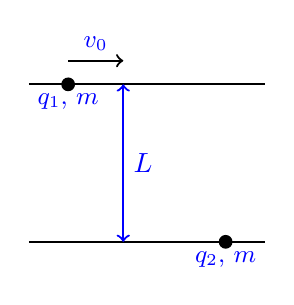
\begin{tikzpicture}
    \draw[thick] (0,0) -- (3,0);
    \draw[thick] (0,2) -- (3,2);
    \draw[blue,<->,thick] (1.2,0) -- (1.2,2) node[midway,right] {$L$};
    \draw[fill=black] (0.5,2) circle (0.08cm) node[below,blue] {\small
      $q_1$, $m$};
    \draw[fill=black] (2.5,0) circle (0.08cm) node[below,blue] {\small
      $q_2$, $m$};
    \draw[thick,->] (0.5,2.3) --++(0.7,0) node[midway,above,blue]
    {\small $v_0$}; 
  \end{tikzpicture}
}

\end{document}


%%% Local Variables: 
%%% mode: latex
%%% TeX-engine:xetex
%%% TeX-PDF-mode: t
%%% End:
